\documentclass[border=1pt, 12pt, tikz]{standalone}

\newcommand\wideOne{3cm}
\newcommand\wideTwo{4cm}
\newcommand\wideThree{2.7cm}
\newcommand\wideFour{3cm}
\newcommand\distOne{2cm}
\newcommand\distTwo{1cm}

\begin{document}
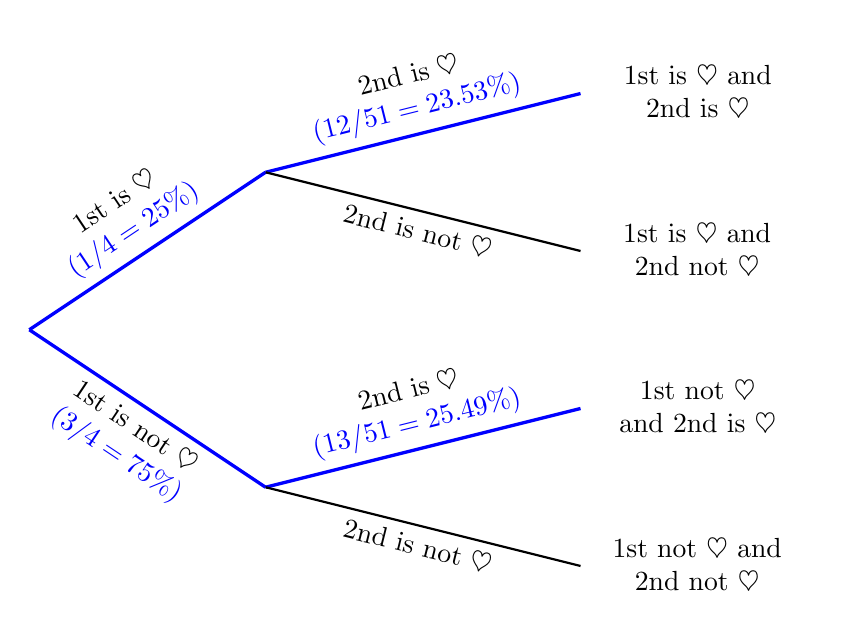
\begin{tikzpicture}[scale=1]

% 1st level
\draw[very thick, blue]%
   (0,0) 
   -- node[above, sloped, align=center]
      {\textcolor{black}{1st is $\heartsuit$}\\$(1/4=25\%)$} 
   (\wideOne,\distOne);
\draw[very thick, blue] 
   (0,0) 
   -- node[below, sloped, align=center]
      {\textcolor{black}{1st is not $\heartsuit$}\\($3/4=75\%$)} 
   (\wideOne,-\distOne);

% 2nd, 3rd and 4th Level
\draw[very thick, blue] 
   (\wideOne,\distOne)
   -- node[above, align=center, sloped]
      {\textcolor{black}{2nd is $\heartsuit$}\\$(12/51=23.53\%)$}
   ++ (\wideTwo,\distTwo) 
      node[right, align=center, text width=\wideThree]
      {\textcolor{black}{1st is $\heartsuit$ and\\2nd is $\heartsuit$}}
   ; 
\draw[thick] 
   (\wideOne,\distOne) 
   -- node[below, align=center, sloped]
      {2nd is not $\heartsuit$}
   ++ (\wideTwo,-\distTwo) 
      node[right, align=center, text width=\wideThree]
      {1st is $\heartsuit$ and 2nd not $\heartsuit$}
   ;
\draw[very thick, blue] 
   (\wideOne,-\distOne) 
   -- node[above, align=center, sloped]
      {\textcolor{black}{2nd is $\heartsuit$}\\$(13/51=25.49\%)$}
   ++ (\wideTwo,\distTwo) 
      node[right, align=center, text width=\wideThree]
      {\textcolor{black}{1st not $\heartsuit$ and 2nd is $\heartsuit$}}
   ;  
\draw[thick] 
   (\wideOne,-\distOne)
   -- node[below, align=center, sloped]
      {2nd is not $\heartsuit$}
   ++ (\wideTwo,-\distTwo) 
      node[right, align=center, text width=\wideThree]
      {1st not $\heartsuit$ and 2nd not $\heartsuit$}
   ; 
\end{tikzpicture}
\end{document}


% \newcommand\wideOne{3cm}
% \newcommand\wideTwo{3.5cm}
% \newcommand\wideThree{2.7cm}
% \newcommand\wideFour{3cm}
% \newcommand\distOne{2cm}
% \newcommand\distTwo{1cm}

% \begin{document}
% \begin{tikzpicture}[scale=1]

% % 1st level
% \draw[thick]%
%    (0,0) 
%    -- node[above, sloped, align=center]
%       {1st is heart} 
%    (\wideOne,\distOne);
% \draw[thick] 
%    (0,0) 
%    -- node[below, sloped, align=center]
%       {1st is not heart} 
%    (\wideOne,-\distOne);

% % 2nd, 3rd and 4th Level
% \draw[thick] 
%    (\wideOne,\distOne)
%    -- node[above, align=center, sloped]
%       {2nd is heart}
%    ++ (\wideTwo,\distTwo) 
%       node[right, align=center, text width=\wideThree]
%       {1st is heart and\\2nd is heart}
%    ; 
% \draw[thick] 
%    (\wideOne,\distOne) 
%    -- node[below, align=center, sloped]
%       {2nd is not heart}
%    ++ (\wideTwo,-\distTwo) 
%       node[right, align=center, text width=\wideThree]
%       {1st is heart and 2nd not heart}
%    ;
% \draw[thick] 
%    (\wideOne,-\distOne) 
%    -- node[above, align=center, sloped]
%       {2nd is heart}
%    ++ (\wideTwo,\distTwo) 
%       node[right, align=center, text width=\wideThree]
%       {1st not heart and 2nd heart}
%    ;  
% \draw[thick] 
%    (\wideOne,-\distOne)
%    -- node[below, align=center, sloped]
%       {2nd is not heart}
%    ++ (\wideTwo,-\distTwo) 
%       node[right, align=center, text width=\wideThree]
%       {1st not heart and 2nd not heart}
%    ; 
% \end{tikzpicture}
% \end{document}
